\section{C\'omo funciona?}

\begin{frame}

\frametitle{C\'omo funciona?}

\begin{columns}
        \begin{column}{.8\textwidth}
        \begin{itemize}
        	\item La aplicaci\'on se comunica con un servidor dedicado para registrar el nuevo usuario, y a 	partir de ese momento env\'ia los datos de geolocalizaci\'on del dispositivo peri\'odicamente.
        \end{itemize}
        \end{column}
        \begin{column}{.2\textwidth}\raggedleft
            
\includegraphics[width=1.5cm]{imagenes/upload.png}
        \end{column}
    \end{columns}

\pause

\begin{columns}
    \begin{column}{.8\textwidth}
    \begin{itemize}
    	\item Cuando el usuario desea consultar el recorrido de un dispositivo, la aplicaci\'on realiza una solicitud al servidor y se muestran las \'ultimas coordenadas recibidas lanzando la aplicaci\'on de mapas del dispositivo.
    \end{itemize}
    \end{column}
    \begin{column}{.2\textwidth}\raggedleft
        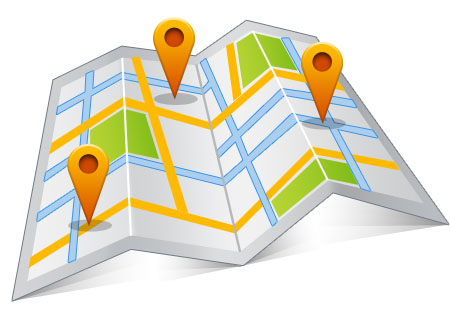
\includegraphics[width=2cm]{imagenes/manypins.png}
    \end{column}
\end{columns}

\pause

\begin{columns}
    \begin{column}{.8\textwidth}
    \begin{itemize}
    	\item Adicionalmente, el dispositivo descarga y muestra tweets con todas las novedades de la aplicaci\'on, publicadas en el Twitter oficial de \textbf{Path Finder}.
    \end{itemize}
    \end{column}
    \begin{column}{.2\textwidth}\raggedleft
        
\includegraphics[width=1.5cm]{imagenes/twitter.png}
    \end{column}
\end{columns}

\end{frame}
